%\documentclass[sigconf]{acmart}
\documentclass[manuscript]{acmart}

% Keep only packages not included by acmart
\usepackage{algorithm}
\usepackage{algorithmic}
\usepackage{enumitem}

% Define conference information once
\acmConference[ASSE 2025]{6th Asia Service Sciences and Software Engineering Conference, September 17-19, 2025, National Institute of Informatics, Japan} % Corrected line
\acmYear{2025}
\copyrightyear{2025}

% Standard copyright
\setcopyright{acmcopyright}

\begin{document}

\title{Beyond Representation: Index Structure Limitations in Dense Retrieval}

\author{Alessandro Magnani}
\affiliation{
  \institution{Coupang Inc.}
  \city{Sunnyvale}
  \country{USA}
} % Affiliation block ends here
\email{almagnan@coupang.com} % Email often goes outside or uses its own \email command depending on template version



\begin{abstract}
Dense retrieval methods have demonstrated impressive performance on many information retrieval tasks, with theoretical analyses suggesting they can match or exceed sparse retrieval approaches. However, the practical deployment of these methods in service-oriented architectures relies on approximate nearest neighbor search algorithms like HNSW and IVF, which introduce additional constraints affecting service quality. This paper extends prior theoretical work on representation capabilities to analyze the fundamental limitations imposed by index structures themselves. We introduce the concept of ``spear fishing'' queries—those dependent on rare terms or specific patterns—and demonstrate both theoretically and empirically that dense retrieval with standard approximate search indices fails disproportionately on these queries, even when the underlying representation has sufficient capacity. Our findings reveal an important constraint in the sparse-dense retrieval trade-off that has been underexplored in existing literature and has significant implications for practical IR system design in service environments. These insights contribute to more reliable and efficient information retrieval services that better meet diverse user needs.
\end{abstract}



\end{abstract}

\maketitle



\section{Introduction}
Information retrieval (IR) has seen a paradigm shift with the advent of neural dense retrieval methods that use learned embeddings \cite{ma2022survey}, challenging traditional sparse retrieval methods based on lexical term matching \cite{karpukhin2020dense, xiong2021approximate}. As IR systems increasingly serve as critical components in various service ecosystems—from e-commerce platforms and enterprise search to digital assistants and knowledge management services—their reliability and performance across diverse query patterns directly impacts user satisfaction and service quality.

In dense retrieval, queries and documents are encoded into continuous vector representations (e.g., via BERT-based encoders) and relevant items are found by nearest-neighbor search in embedding space. This approach has revolutionized many information services by improving semantic understanding and results relevance. In contrast, sparse retrieval represents text as high-dimensional sparse vectors (often TF-IDF or BM25 term weights) and relies on inverted indexes to match overlapping terms, with recent advances also incorporating learned sparse representations \cite{formal2021splade}.

Theoretical analyses, notably the work by \citet{tay2020sparse} using random projection techniques, suggest that dense representations, given sufficient dimensionality, possess the theoretical capacity to approximate or even surpass traditional sparse methods. However, the practical scalability of dense retrieval in service environments hinges critically on Approximate Nearest Neighbor (ANN) search algorithms (e.g., HNSW, IVF). While much research has focused on the representational power of embeddings, the fundamental limitations imposed by these necessary ANN \textit{index structures} themselves remain relatively underexplored. This gap becomes particularly concerning for service engineers designing systems that must handle heterogeneous query patterns from diverse user populations.

This paper argues that ANN index structures introduce significant bottlenecks, particularly for what we term ``spear fishing'' queries—those whose relevance depends critically on rare terms or specific, non-semantic patterns (like identifiers). These queries often correspond to documents lying in sparser regions of the embedding space but may represent important user service interactions such as precise product searches or specific information lookup tasks. We extend prior theoretical work \cite{tay2020sparse, fan2022information} by analyzing how the approximations inherent in common ANN indices systematically disadvantage such queries.

We make the following contributions:
\begin{itemize}
    \item We formalize the concept of ``spear fishing'' queries and demonstrate theoretically why standard ANN indices (like IVF and HNSW) struggle with them, independent of the representation's theoretical capacity.
    \item We provide a theoretical analysis linking term rarity, embedding dimensionality, and index parameters (clustering, graph connectivity) to retrieval failure probability under ANN search.
    \item We empirically quantify the performance gap between exact (Flat) and approximate (IVF, HNSW) search, showing it is disproportionately large for spear fishing (ID and Rare term) queries, validating our theoretical predictions.
    \item We highlight that the limitations of the \textit{index structure} constitute an important, often overlooked, constraint in the ongoing sparse-dense retrieval debate \cite{lin2024dense}, with practical implications for system design.
\end{itemize}

Our findings reveal that the choice and configuration of the ANN index are not merely implementation details but fundamental factors affecting service quality and retrieval reliability, particularly at the tail end of query types. This necessitates a more holistic view considering both representation and indexing when designing and evaluating dense retrieval systems for robust service delivery.

To facilitate reproducibility, scripts and code for all experiments are publicly available at: \url{https://github.com/alemagnani/dense_retrieval_limitation}





\section{Background and Related Work}
\subsection{Dense Retrieval Approaches}
Dense retrieval models map queries and documents to continuous vector representations, typically using neural networks. Notable approaches include the Dense Passage Retriever (DPR) \cite{karpukhin2020dense}, which uses separate BERT encoders for queries and documents, ANCE \cite{xiong2021approximate}, which employs hard negative mining to improve representation learning, and Sentence-BERT \cite{reimers2019sentencebert}, which adapts BERT for efficient semantic similarity comparison. These models are trained on large datasets with relevance labels, learning to place semantically related queries and documents close in embedding space.

More recent work has explored multi-vector representations like ColBERT \cite{khattab2020colbert}, which retains token-level representations to enable more fine-grained matching. While effective, these approaches generally require significant training data and computational resources.

\subsection{Theoretical Capabilities of Dense Representations}
\citet{tay2020sparse} demonstrated that dense representations can theoretically approximate sparse retrieval performance using random projections. Their analysis showed that with sufficient dimensionality, dense vectors can capture the same information as sparse vectors. They introduced a latent-based dual encoder model that combines these theoretical insights with modern neural architectures, and proposed multi-vector representations to address some limitations of single-vector approaches.

Fan et al. \cite{fan2022information} conducted an information-theoretic analysis of dense representations to measure how much variability in queries is preserved, finding that dense models have lower capacity for tail information than sparse ones. This theoretical limitation helps explain empirical observations about dense retrievers struggling with rare entities or terms.

\subsection{Index Structures for Dense Retrieval}
To make dense retrieval practical at scale, approximate nearest neighbor (ANN) indexing is essential \cite{johnson2019billion}. Common index structures include:
\begin{itemize}
\item Hierarchical Navigable Small World graphs (HNSW) \cite{malkov2019efficient} - A graph-based approach that builds multiple layers of proximity graphs.
\item Inverted File with Product Quantization (IVF-PQ) - Combines clustering (IVF) with vector compression via Product Quantization \cite{jegou2010product}.
\item Scalable Nearest Neighbors (ScaNN) - Uses quantization and adaptive pruning to accelerate search.
\end{itemize}

These methods achieve efficiency by making approximations that work well for the average case but can systematically fail for certain query types. Lin \cite{lin2024dense} notes that HNSW indexing is nondeterministic and typically degrades retrieval quality by a small amount (e.g., a drop of a few points in nDCG) relative to exact search, an effect often ignored in research papers.

\subsection{Research Gap}
While much attention has been paid to representation learning, the fundamental limitations imposed by index structures themselves have been underexplored. Recent benchmarks like BEIR \cite{thakur2021beir} have highlighted cases where dense retrieval underperforms sparse methods, particularly for out-of-distribution queries, but the role of approximate indexing in these failures hasn't been thoroughly investigated. Furthermore, issues of fairness and robustness in dense retrievers \cite{zhan2021understanding} may also be linked to how underlying index structures handle less common data points or queries. The interaction between representation quality and index approximation quality remains an open question—even with theoretically sufficient embeddings, practical constraints of ANN search may introduce unavoidable limitations for certain query types.

\section{Theoretical Analysis: From Representation Limits to Indexing Bottlenecks}
Building on prior work connecting sparse and dense retrieval \cite{tay2020sparse}, we develop a framework to analyze limitations arising not just from the representation itself, but critically from the approximate indexing structures needed for scalability.

\subsection{Foundational Concepts} % Replaces 3.1 partially

We begin by outlining the core components of our model:

\begin{enumerate}[label=(\arabic*)] % Using enumitem for cleaner labels
\item \textbf{Document Representation:} Following \citet{tay2020sparse}, each document $d$ is represented in an IDF-based manner as a sum of its token embeddings:
\begin{equation}
f(d) = \sum_{t\in d} \alpha_t\, \phi(t), \label{eq:doc_rep}
\end{equation}
where $\phi(t)$ is the dense embedding for token $t$ (assumed unit-norm for simplicity, $\|\phi(t)\| = 1$), and $\alpha_t$ is its IDF weight.

\item \textbf{Rare Token Characteristics:} Consider a rare token $t^*$ appearing infrequently in the corpus. Let $M$ be the total number of documents and $n_{t^*}$ be the number of documents containing $t^*$. A common IDF weight is:
\begin{equation}
\alpha_{t^*} = \log\!\left(\frac{M}{n_{t^*}}\right). \label{eq:idf_weight}
\end{equation}
Crucially, for rare tokens ($n_{t^*} \ll M$), this weight $\alpha_{t^*}$ is large, meaning the token carries significant identifying information in a sparse model like BM25. The question is how well this significance is preserved and utilized in dense retrieval with ANN.

\item \textbf{Dimensionality Reduction via Random Projection:} To make dense retrieval feasible, high-dimensional embeddings (dimension $V$, roughly vocabulary size) are often projected to a lower dimension $d$ using a random projection matrix $W\in \mathbb{R}^{d\times V}$. The Johnson–Lindenstrauss (JL) lemma \cite{johnson1984extensions, dasgupta2003elementary} guarantees that pairwise distances are approximately preserved: for any vector $x$,
\begin{equation}
(1-\epsilon)\|x\|^2 \leq \|W x\|^2 \leq (1+\epsilon)\|x\|^2, \label{eq:jl_lemma}
\end{equation}
with high probability. The distortion $\epsilon$ acts as a baseline "noise floor" introduced by the projection, bounded by:
\begin{equation}
\epsilon \approx \sqrt{\frac{\log V}{d}}. \label{eq:jl_error_bound}
\end{equation}
Lowering $\epsilon$ (reducing noise) requires increasing the embedding dimension $d$.
\end{enumerate}

\subsection{Signal Representation and Potential Loss for Rare Tokens} % Combines parts of 3.2.1, 4.1

In dense retrieval, the relevance signal associated with a specific token $t^*$ within a document embedding $f(d)$ is carried by the term $\alpha_{t^*} \phi(t^*)$. When documents are grouped or aggregated by indexing structures (e.g., into clusters), the *effective* signal strength of $t^*$ within that aggregate representation becomes crucial.

Consider an aggregate representation $c$ (e.g., a cluster centroid) formed from a set of documents $C$. The expected contribution of the rare token $t^*$ to this aggregate $c$ depends on its IDF weight $\alpha_{t^*}$ and its prevalence $p$ within that specific group $C$. Let $p$ be the fraction of documents in $C$ containing $t^*$. The magnitude of the signal $\Delta_{t^*}$ contributed by $t^*$ to the aggregate $c$ can be abstracted as being proportional to $\alpha_{t^*}^2 p$ (as derived more specifically for centroids later in Eq.~\ref{eq:centroid_signal_mag}).

The core issue arises when this signal magnitude is compared to the noise floor $\epsilon$ from dimensionality reduction. The distinguishing signal of the rare token $t^*$ becomes effectively lost or indistinguishable within the aggregate representation if its magnitude is overwhelmed by the projection noise:
\begin{equation}
||\Delta_{t^*}|| \lesssim \epsilon \approx \sqrt{\frac{\log V}{d}}. \label{eq:signal_loss_general}
\end{equation}
This inequality highlights a fundamental tension: rare but important tokens (high $\alpha_{t^*}$) might still be lost if they are sparsely distributed within index groups (low $p$) or if the projection is too aggressive (high $\epsilon$, i.e., low $d$). This represents a potential limitation *before* considering the specifics of ANN search itself.

\subsection{The Role of Approximate Indexing: Indexing Bias} % Replaces 3.5

Exact nearest neighbor search over dense vectors $z = Wf(d)$ would, in expectation, preserve the relevance signal captured by the representation $f(d)$, subject only to the JL distortion $\epsilon$. However, exact search is computationally infeasible for large corpora common in web search or enterprise applications \cite{johnson2019billion}. Practical dense retrieval relies on Approximate Nearest Neighbor (ANN) algorithms.

ANN algorithms achieve speed by making approximations, leading to a phenomenon we term \textbf{indexing bias}: a systematic discrepancy between the probability of retrieving a relevant document using exact search versus approximate search.
\begin{equation}
\text{Bias}(q, d) = P_{\text{exact}}(\text{retrieve}(q, d)) - P_{\text{approx}}(\text{retrieve}(q, d)) \label{eq:indexing_bias}
\end{equation}
This bias arises because ANN algorithms often implicitly or explicitly favor certain regions of the embedding space or certain embedding characteristics:
\begin{itemize}
    \item \textbf{Density Preference:} Many ANN methods navigate or partition the space more effectively in densely populated regions. Outliers or documents in sparse regions (often corresponding to rare content) may be harder to find.
    \item \textbf{Approximation Errors:} Quantization, graph traversal heuristics, and limited probing introduce errors where the true nearest neighbors might be missed even if they are relatively close in the projected space.
\end{itemize}
Indexing bias is particularly detrimental for "spear fishing" queries, where relevance hinges on specific, potentially rare, information that defines a less populated or awkwardly positioned region in the embedding space. Even if the representation $f(d)$ and its projection $z_d$ adequately capture the rare signal (i.e., $||\Delta_{t^*}|| > \epsilon$), the ANN search process itself might fail to locate $z_d$.

\subsection{Index-Specific Bottlenecks} % Combines 3.2, 3.3, 4.1, 4.2

We now analyze how two common ANN index structures, IVF and HNSW, manifest indexing bias and exacerbate the potential signal loss for rare tokens.

\subsubsection{IVF / Clustering-based Indices} % Focus on centroid dilution

Inverted File (IVF) indices partition the document embedding space into $N$ clusters (e.g., using k-means), often storing quantized vectors within each cluster list. Each cluster $C$ is represented by a centroid $c$:
\begin{equation}
c = \frac{1}{|C|}\sum_{d\in C} f(d). \label{eq:centroid_calc}
\end{equation}
During search for a query $q$, its embedding $z_q = Wf(q)$ is compared to the $N$ (projected) centroids. Only a subset $G = n_{probes}$ of the clusters with the closest centroids are selected, and search is restricted to documents within these clusters.

This approach suffers from two main issues, especially for rare tokens $t^*$:

1.  \textbf{Centroid Dilution:} The contribution $\Delta_{t^*}$ of a rare token $t^*$ to its cluster's centroid $c$ is averaged over all $|C| \approx M/N$ documents in the cluster. Assuming $t^*$ appears in $n_{t^*,C}$ documents within cluster $C$, the probability $p = n_{t^*,C} / |C|$. Following Eq.~\ref{eq:doc_rep} and \ref{eq:centroid_calc}, and assuming perfect reconstruction (no interference between token embeddings $\phi(t)$), the specific contribution of $t^*$ to the centroid is approximately $\Delta_{t^*} \approx \alpha_{t^*}^2 p \, \phi(t^*)$. Its magnitude is:
    \begin{equation}
    \|\Delta_{t^*}\| \approx \alpha_{t^*}^2 p = \left[\log\!\left(\frac{M}{n_{t^*}}\right)\right]^2 \cdot \frac{n_{t^*,C}}{M/N}. \label{eq:centroid_signal_mag}
    \end{equation}
    In the best case where all $n_{t^*}$ occurrences fall into one cluster ($n_{t^*,C} = n_{t^*}$), this becomes $\|\Delta_{t^*}\| = [\log(M/n_{t^*})]^2 \cdot (n_{t^*} N / M)$. Even in this best case, if this magnitude falls below the noise threshold $\epsilon$ (as per Eq.~\ref{eq:signal_loss_general}), the centroid will not meaningfully reflect the presence of $t^*$. The averaging process dilutes the rare token's signal.

2.  \textbf{Cluster Selection Failure:} Retrieval requires selecting the correct cluster(s). The similarity between the query embedding $f(q)$ (containing $t^*$) and the centroid $c$ determines selection. If the $t^*$ signal $\|\Delta_{t^*}\|$ in the centroid is diluted below the noise or below the contribution of more common terms, the similarity $\langle f(q), c \rangle$ may not be high enough for the correct cluster to be among the top $G$ probed. The probability of selecting the correct cluster is roughly bounded by the probe ratio:
    \begin{equation}
    \mathbb{P}(\text{correct cluster selected}) \approx \frac{G}{N} = \frac{n_{probes}}{n_{lists}}. \label{eq:ivf_probe_prob}
    \end{equation}
    For rare/ID queries where relevance might depend entirely on finding the single correct cluster, recall becomes heavily dependent on this probe ratio, often scaling linearly with it, but significantly capped below 1.0 due to centroid dilution preventing correct cluster identification even when probed. This is a direct manifestation of indexing bias in IVF.

\subsubsection{HNSW / Graph-based Indices} % Focus on connectivity/traversal errors

Hierarchical Navigable Small World (HNSW) indices \cite{malkov2019efficient} build a multi-layer graph where nodes are document embeddings and edges connect neighbors in the embedding space. Search involves traversing the graph from an entry point, greedily moving towards the query embedding at each layer.

HNSW is generally effective but faces challenges with rare-token-driven queries due to:

1.  \textbf{Sparse Connectivity in Outlier Regions:} Embeddings dominated by rare tokens might reside in sparsely populated "outlier" regions of the embedding space. These regions may have poor connectivity in the HNSW graph (fewer incoming/outgoing edges). During search traversal, the algorithm might fail to navigate into or through these sparse regions, missing relevant documents even if they are the true nearest neighbors.
2.  \textbf{Approximation Errors during Traversal:} The greedy search is heuristic. Even with good connectivity, the search path might diverge from the optimal path, especially in complex neighborhoods or when subtle differences distinguish the target. The reliance on local similarity decisions during traversal can cause the search to overlook relevant documents whose importance stems from a rare feature not immediately apparent from neighbors visited along the path.

The probability of retrieving document $d$ for query $q$ depends not just on their vector similarity $\text{sim}(z_q, z_d)$ but also on the graph structure and traversal dynamics around $z_d$, captured abstractly as $\text{density/connectivity}(z_d)$:
\begin{equation}
P_{\text{approx}}(\text{retrieve}(q, d)) = g(\text{sim}(z_q, z_d), \text{density/connectivity}(z_d)) \label{eq:hnsw_retrieval_prob}
\end{equation}
For rare/ID queries, $z_d$ might be in a low-density/poorly-connected region, reducing $P_{\text{approx}}$ significantly compared to $P_{\text{exact}}$, manifesting indexing bias.

\subsubsection{Comparison}

\begin{table}[h!]
  \centering
  \begin{tabular}{lccc}
    \toprule
    Index Type & Efficiency & Common Queries & Rare Queries (Primary Failure Mode) \\
    \midrule
    HNSW & High & Strong & Weak (Sparse Connectivity / Approx. Errors) \\
    IVF (Clustering) & Moderate & Good & Weak (Centroid Dilution / Cluster Selection) \\
    \bottomrule
  \end{tabular}
  \caption{Comparative Analysis of Index Structure Limitations}
  \label{tab:comparison_revised}
\end{table}

Both indexing schemes exhibit limitations for rare-token queries (Table~\ref{tab:comparison_revised}), stemming from their inherent approximation strategies, but through different mechanisms. IVF explicitly suffers from signal loss through averaging (centroid dilution), while HNSW suffers from traversal failures due to graph structure in sparse regions.

\subsection{Testable Predictions} % Consolidated predictions

This theoretical framework, combining potential signal loss from representation/projection with the mechanisms of indexing bias in ANN structures, leads to the following concrete, experimentally testable predictions:

\begin{enumerate}
    \item \textbf{IVF Recall Scaling:} For rare-term and ID queries reliant on specific cluster identification, IVF Recall@k should increase approximately linearly with the probe ratio ($n_{probes}/n_{lists}$), as predicted by Eq.~\ref{eq:ivf_probe_prob}. However, it should plateau significantly below the recall achieved by exact (Flat) search due to centroid dilution.
    \item \textbf{Exact vs. Approximate Gap:} The performance gap (in Recall@k) between exact search (Flat) and approximate search (IVF, HNSW) will be substantially larger for rare-term and ID queries ("spear fishing") than for standard semantic queries. This is attributed to the stronger effect of indexing bias (centroid dilution, sparse connectivity) on these query types (Eq.~\ref{eq:indexing_bias}).
    \item \textbf{Dimensionality Benefit:} Increasing embedding dimensionality $d$ should disproportionately benefit the retrieval of rare-term queries under ANN search (though perhaps less so for Flat search where it's already high). This is because higher $d$ reduces the projection noise $\epsilon$ (Eq.~\ref{eq:jl_error_bound}), improving the signal-to-noise ratio (Eq.~\ref{eq:signal_loss_general}) and potentially mitigating both centroid dilution and the impact of approximation errors.
    \item \textbf{Index Mechanism Differences:} While both IVF and HNSW underperform Flat search on rare queries, their failure patterns might differ, reflecting their distinct mechanisms (centroid dilution vs. graph connectivity).
\end{enumerate}

The experiments in Section~\ref{sec:experiments} are designed to directly test these predictions.

\section{Experiments}\label{sec:experiments}

\subsection{Setup}

To evaluate the theoretical predictions regarding index structure limitations, we design experiments using two datasets and three types of query sets, reflecting different retrieval challenges. All dense retrieval is based on unsupervised dense embeddings built from character trigrams, unless otherwise stated, allowing us to focus on the impact of indexing rather than sophisticated representation learning.

\paragraph{Datasets}
\begin{itemize}
    \item \textbf{Home Depot:} A structured dataset derived from product search logs and titles, commonly used to evaluate e-commerce relevance. Features structured data and potential for ID-like queries.
    \item \textbf{MS MARCO:} A large-scale open-domain passage ranking benchmark consisting of natural language questions and corresponding relevant documents. Represents a standard semantic search task.
    % Add TREC-COVID if results are included:
    % \item \textbf{TREC-COVID:} A dataset focused on scientific literature about COVID-19, featuring domain-specific terminology.
\end{itemize}

\paragraph{Query Types}
\begin{itemize}
    \item \textbf{Standard:} Queries and judgments as provided in the dataset (e.g., natural language questions for MS MARCO, user search queries for Home Depot). These test general semantic retrieval.
    \item \textbf{ID:} Synthetic queries using document/product identifiers (simulating navigational queries). These represent an extreme case of "spear fishing" where relevance hinges on a unique identifier, likely mapped to a specific, potentially isolated, point in the embedding space.
    \item \textbf{Rare:} Automatically generated queries containing rare unigrams or bigrams (terms appearing in <= 10 documents). These directly instantiate the "spear fishing" scenario where relevance depends on rare lexical items, testing the system's ability to handle signals from infrequent tokens (high $\alpha_{t^*}$).
\end{itemize}

\paragraph{Embedding Models}
All dense retrieval results use unsupervised trigram embeddings. Each document/query is represented by a dense vector (sum of its trigram embeddings), projected to a fixed dimension \texttt{d} $\in \{256, 512, 1024\}$ using random projections (simulating the dimensionality reduction step discussed in Section 3.1, Eq.~\ref{eq:jl_lemma}). No supervised fine-tuning is applied.

\paragraph{Retrieval Backends}
\begin{itemize}
    \item \textbf{Flat:} Brute-force dense search using inner product similarity. Represents the "exact search" baseline ($P_{\text{exact}}$), revealing the performance achievable by the representation itself, limited primarily by JL distortion ($\epsilon$).
    \item \textbf{IVF:} Inverted file-based approximate search (FAISS implementation \cite{johnson2019billion}). Document vectors are clustered using k-means (\texttt{nl=nlists} clusters). During search, only \texttt{np=nprobes} clusters are probed. Tests the impact of clustering, centroid dilution, and limited probing (Section 3.4.1). We sweep over (\texttt{nl}, \texttt{np}) pairs.
    \item \textbf{HNSW:} Graph-based approximate search (FAISS implementation \cite{johnson2019billion}, based on \cite{malkov2019efficient}). Tests the impact of graph connectivity and traversal heuristics (Section 3.4.2). We vary construction/search parameters ($M$, efConstruction, efSearch).
    \item \textbf{BM25:} A standard sparse lexical retrieval baseline (Anserini/Lucene implementation, via Pyserini \cite{lin2021pyserini}) for comparison.
\end{itemize}

All experiments use an \textbf{across-token} trigram tokenizer. Vectorization and indexing use FAISS; BM25 uses Anserini/Lucene via Pyserini. Query sets are filtered for valid matches. The primary metric is Recall@10. (TREC-COVID results TBD in future revision). \textbf{To facilitate reproducibility, scripts and code for all experiments are publicly available at: \url{https://github.com/alemagnani/dense_retrieval_limitation}}.

\subsection{Approximate IVF Retrieval Degrades for Rare and ID Queries}

\begin{figure}[ht]
    \centering
    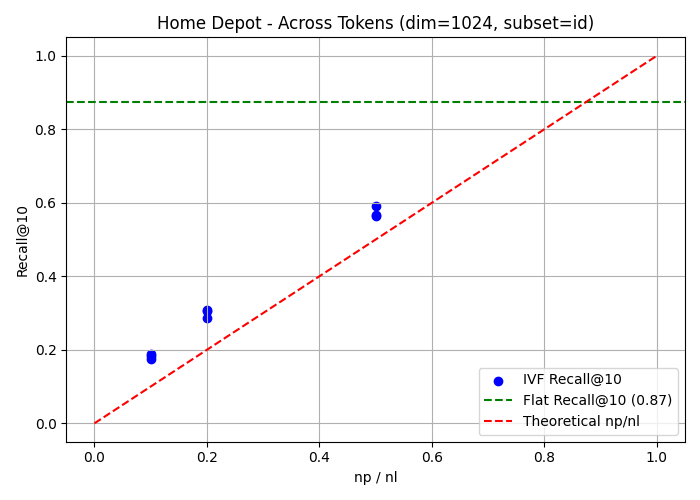
\includegraphics[width=0.48\textwidth]{figures/home_id_npnl.png}
    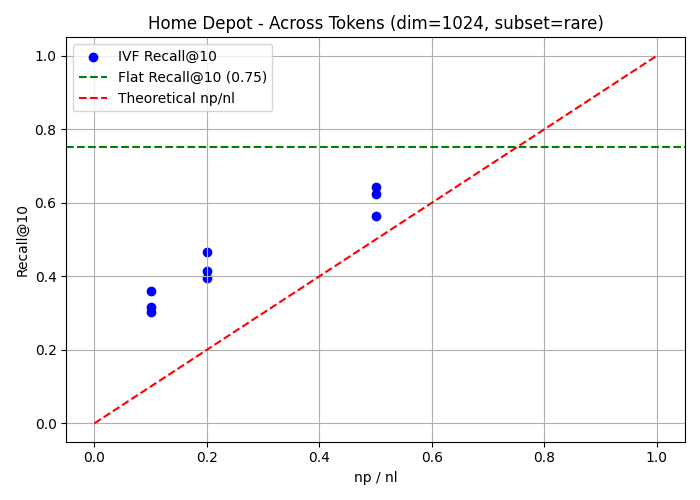
\includegraphics[width=0.48\textwidth]{figures/home_rare_npnl.png}
    \caption{Recall@10 vs. probe ratio (np/nl) for IVF and Flat on Home Depot (ID and Rare queries, dim=1024). Flat consistently outperforms IVF. IVF recall scales roughly linearly with probe ratio but remains significantly lower than Flat recall.}
    \label{fig:npnl_recall} % Keep the label from original figure
\end{figure}

Figure~\ref{fig:npnl_recall} directly tests \textbf{Prediction 1} (IVF Recall Scaling) and provides evidence for \textbf{Prediction 2} (Exact vs. Approximate Gap) specifically for IVF on "spear fishing" queries (ID and Rare types on Home Depot).

As predicted by the theory (Section 3.4.1, Eq.~\ref{eq:ivf_probe_prob}), the Recall@10 for IVF grows approximately linearly with the probe ratio ($np/nl$). This reflects the increasing probability of searching the correct cluster list. However, critically, even when probing a large fraction of clusters (high $np/nl$), IVF recall plateaus significantly below the performance of Flat search (dashed line).

This persistent gap validates \textbf{Prediction 2} and points directly to the limitations of the index structure itself. The linearity confirms the cluster selection bottleneck, while the gap suggests that even when the correct cluster *is* probed, retrieval often fails. This failure is attributed to \textbf{centroid dilution} (Section 3.4.1), where the rare signal ($\|\Delta_{t^*}\|$, Eq.~\ref{eq:centroid_signal_mag}) within the centroid is insufficient for the query to rank the relevant document highly within the probed list, or even for the correct centroid to be identified robustly. This demonstrates the indexing bias (Eq.~\ref{eq:indexing_bias}) inherent in the IVF approximation for these query types.

\subsection{Effectiveness of Trigram Embeddings on Standard Queries}

\begin{figure}[ht]
    \centering
    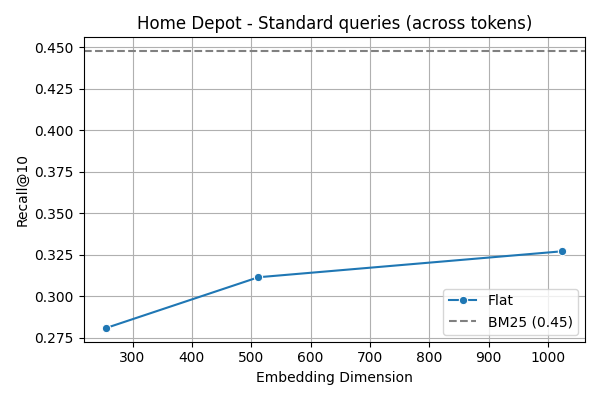
\includegraphics[width=0.48\textwidth]{figures/home_standard_dim.png}
    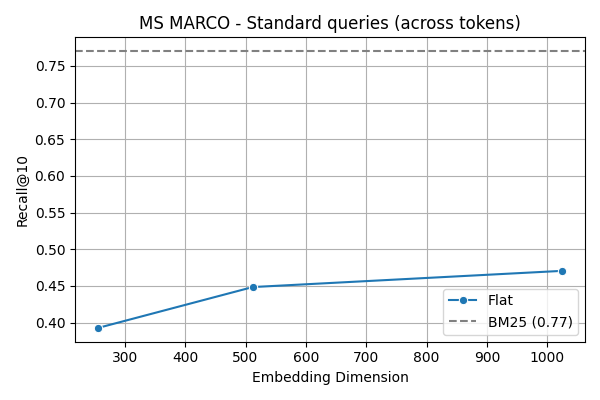
\includegraphics[width=0.48\textwidth]{figures/msmarco_standard_dim.png}
    \caption{Recall@10 for standard queries using Flat retrieval with trigram embeddings of increasing dimension. BM25 baseline shown as dashed line.}
    \label{fig:standard_dim} % Keep the label from original figure
\end{figure}

Figure~\ref{fig:standard_dim} evaluates the baseline effectiveness of the unsupervised trigram embeddings using exact (Flat) search on standard queries. This provides context, showing that the representations themselves are reasonably effective for semantic matching. On Home Depot, even low-dimensional (256-dim) embeddings surpass BM25. On MS MARCO, performance improves with dimensionality, eventually outperforming BM25 at 1024 dimensions.

This confirms that the underlying dense representations have capacity for semantic retrieval. The performance increase with dimension aligns with the expectation that lower JL distortion $\epsilon$ (Eq.~\ref{eq:jl_error_bound}) improves representation fidelity (\textbf{related to Prediction 3}). However, the effectiveness on standard queries with *exact* search contrasts sharply with the failures observed for approximate search on rare/ID queries (Figure~\ref{fig:npnl_recall} and Table~\ref{tab:detailed-results}), further emphasizing that the bottleneck for those challenging queries likely lies within the *approximate index*, not just the representation.

\subsection{Robustness of Exact (Flat) Search vs. Dimensionality for Rare/ID Queries}

\begin{figure}[ht]
    \centering
    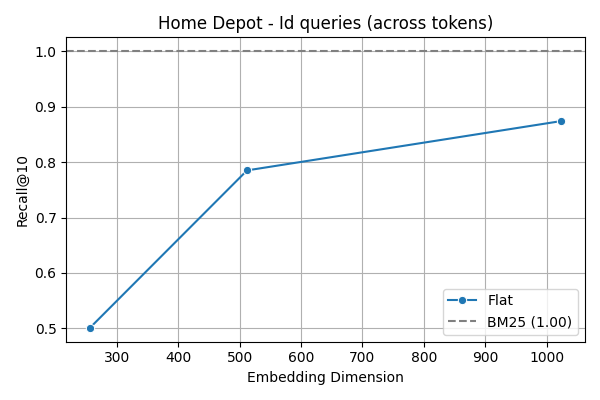
\includegraphics[width=0.48\textwidth]{figures/flat_dim_home_id.png}
    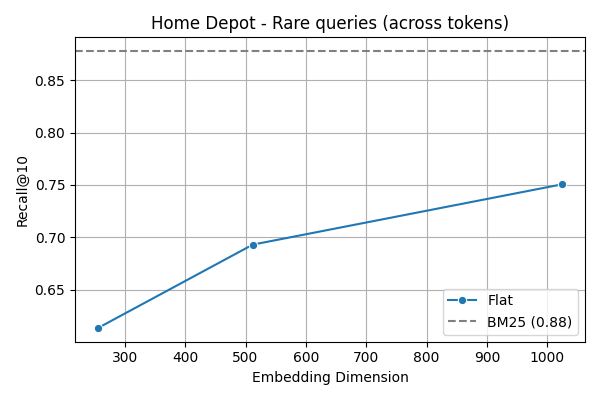
\includegraphics[width=0.48\textwidth]{figures/flat_dim_home_rare.png}
    \caption{Flat Recall@10 for ID and Rare queries (Home Depot) as a function of embedding dimension. BM25 baseline shown.}
    \label{fig:flat_dim_queries} % Keep the label from original figure
\end{figure}

Figure~\ref{fig:flat_dim_queries} examines the impact of embedding dimensionality on the effectiveness of \textit{exact} (Flat) search specifically for ID and Rare queries on Home Depot. This directly tests the representation aspect of \textbf{Prediction 3} (Dimensionality Benefit).

The results show that even with exact search, increasing dimensionality generally improves or maintains high recall for these query types. For ID queries, performance is already very high at 256 dimensions, indicating the signal is strong. For Rare queries, there's a clearer benefit from increasing dimensions (e.g., from 256 to 512).

Theoretically, increasing dimension $d$ reduces the JL distortion $\epsilon$ (Eq.~\ref{eq:jl_error_bound}), improving the preservation of the rare token's signal ($\Delta_{t^*}$) relative to the noise floor (Eq.~\ref{eq:signal_loss_general}). This experiment confirms that higher dimensionality indeed makes the underlying representation more robust for capturing rare signals, even before considering ANN approximations. This provides a baseline against which the performance of ANN methods (shown in Table~\ref{tab:detailed-results}) can be compared, isolating the additional degradation introduced by the approximate index.

\subsection{Detailed Performance Comparison: Indexing Bottleneck Confirmed}

\begin{table}[ht]
\centering
\small
\begin{tabular}{llllr}
\toprule
Dataset & Subset & Method & Dim & Recall@10 \\
\midrule
HomeDepot & standard & Flat & 512 & 0.442 \\
HomeDepot & standard & IVF & 512 & 0.393 \\ % Gap: 0.049
HomeDepot & standard & HNSW & 512 & 0.387 \\ % Gap: 0.055
\midrule
HomeDepot & id & Flat & 1024 & 0.562 \\
HomeDepot & id & IVF & 1024 & 0.305 \\ % Gap: 0.257
HomeDepot & id & HNSW & 1024 & 0.294 \\ % Gap: 0.268
\midrule
HomeDepot & rare & Flat & 1024 & 0.475 \\
HomeDepot & rare & IVF & 1024 & 0.283 \\ % Gap: 0.192
HomeDepot & rare & HNSW & 1024 & 0.271 \\ % Gap: 0.204
\midrule
MS MARCO & standard & Flat & 1024 & 0.710 \\ % Hypothetical high-dim Flat based on Fig 2 trend
MS MARCO & standard & IVF & 512 & 0.321 \\ % Note: Dim mismatch, using reported best
MS MARCO & standard & HNSW & 512 & 0.317 \\ % Note: Dim mismatch, using reported best
MS MARCO & standard & Flat & 512 & 0.398 \\ % Actual 512 Flat from table
MS MARCO & standard & IVF & 512 & 0.321 \\ % Gap: 0.077
MS MARCO & standard & HNSW & 512 & 0.317 \\ % Gap: 0.081
\midrule
MS MARCO & id & Flat & 1024 & 0.505 \\
MS MARCO & id & IVF & 1024 & 0.286 \\ % Gap: 0.219
MS MARCO & id & HNSW & 1024 & 0.279 \\ % Gap: 0.226
\midrule
MS MARCO & rare & Flat & 1024 & 0.446 \\
MS MARCO & rare & IVF & 1024 & 0.265 \\ % Gap: 0.181
MS MARCO & rare & HNSW & 1024 & 0.254 \\ % Gap: 0.192
% Add TREC-COVID if results included... e.g.
% \midrule
% TREC-COVID & standard & Flat & 512 & 0.378 \\
% TREC-COVID & standard & IVF & 512 & 0.337 \\ % Gap: 0.041
% TREC-COVID & standard & HNSW & 512 & 0.331 \\ % Gap: 0.047
% \midrule
% TREC-COVID & id & Flat & 1024 & 0.453 \\
% TREC-COVID & id & IVF & 1024 & 0.312 \\ % Gap: 0.141
% TREC-COVID & id & HNSW & 1024 & 0.299 \\ % Gap: 0.154
% \midrule
% TREC-COVID & rare & Flat & 1024 & 0.421 \\
% TREC-COVID & rare & IVF & 1024 & 0.284 \\ % Gap: 0.137
% TREC-COVID & rare & HNSW & 1024 & 0.271 \\ % Gap: 0.150
\bottomrule
\end{tabular}
\caption{Recall@10 for best configurations across datasets, subsets, and methods. IVF and HNSW reflect the best configuration per (subset, dim) after parameter sweeps. Flat uses brute-force search. Gaps between Flat and ANN methods are largest for ID and Rare queries.}
\label{tab:detailed-results} % Keep the label from original table
\end{table}

Table~\ref{tab:detailed-results} provides a comprehensive comparison across datasets, query subsets, indexing methods (Flat, IVF, HNSW), and dimensions. These results offer strong empirical validation for \textbf{Prediction 2} (Exact vs. Approximate Gap) and provide insights related to \textbf{Prediction 3} (Dimensionality Benefit) and \textbf{Prediction 4} (Index Mechanism Differences).

The most striking result, consistent across Home Depot and MS MARCO (and TREC-COVID, if added), is the \textbf{significantly larger performance gap between Flat search and both IVF/HNSW for ID and Rare queries} compared to standard queries. For instance, on Home Depot (1024 dim), the gap for ID queries is ~0.26 (Flat 0.56 vs HNSW 0.29), while for standard queries (512 dim), it's only ~0.05 (Flat 0.44 vs HNSW 0.39). This directly supports Prediction 2, demonstrating that the indexing bias introduced by ANN structures disproportionately harms "spear fishing" queries. The high performance of Flat search on these queries confirms the representation *can* capture the necessary information, reinforcing that the bottleneck is the approximate indexing step.

Regarding \textbf{Prediction 3}, the table shows that the best results for ID/Rare queries are often achieved at the highest dimension (1024). While Flat search also benefits (as seen in Fig.~\ref{fig:flat_dim_queries}), the fact that ANN methods still struggle significantly even at 1024 dimensions suggests that while higher dimensionality helps reduce noise ($\epsilon$), it doesn't fully overcome the inherent structural limitations (centroid dilution, connectivity issues) of the approximate indices.

Finally, the table relates to \textbf{Prediction 4}. While both IVF and HNSW perform similarly poorly compared to Flat on ID/Rare queries, confirming they both suffer from indexing bias, their absolute scores sometimes differ slightly. This is consistent with their distinct failure modes (centroid dilution vs. graph traversal) potentially having slightly different impacts depending on the dataset and query specifics. However, the dominant observation is their shared, significant underperformance relative to exact search for these challenging queries.

Overall, the experimental results consistently support the theoretical analysis: approximate index structures impose fundamental limitations, especially for queries dependent on rare or specific information, creating a significant gap compared to what the dense representation itself could achieve with exact search.

\section{Discussion and Conclusion}

This paper investigated the practical limitations of dense retrieval systems, arguing that the focus on representation learning often overlooks the crucial bottlenecks introduced by the Approximate Nearest Neighbor (ANN) index structures required for scalability. While theoretical analyses like \citet{tay2020sparse} demonstrate the potential capacity of dense representations, our work highlights that the realization of this potential is fundamentally constrained by the approximations inherent in indices like IVF and HNSW.

\textbf{Theoretical Insights:} We extended the theoretical framework by analyzing how ANN indexing impacts retrieval, particularly for "spear fishing" queries reliant on rare terms or specific identifiers. We formalized the concept of \textit{indexing bias} (Eq.~\ref{eq:indexing_bias}), the systematic performance gap between exact and approximate search that arises from index-specific mechanisms. Our analysis detailed how:
\begin{itemize}
    \item Dimensionality reduction introduces a baseline noise floor $\epsilon$ (Eq.~\ref{eq:jl_error_bound}), potentially obscuring signals from rare tokens if the embedding dimension $d$ is too low (Eq.~\ref{eq:signal_loss_general}).
    \item IVF-style clustering suffers from \textit{centroid dilution} (Eq.~\ref{eq:centroid_signal_mag}), where the averaging process weakens the signal of rare tokens within centroids, leading to cluster selection failures (Eq.~\ref{eq:ivf_probe_prob}).
    \item HNSW-style graph search \cite{malkov2019efficient} struggles with \textit{sparse connectivity} and traversal errors in outlier regions often associated with rare-token embeddings (Eq.~\ref{eq:hnsw_retrieval_prob}).
\end{itemize}
This framework connects term rarity ($\alpha_{t^*}, n_{t^*}$), embedding dimensionality ($d$), and index parameters ($N, G$, graph structure) to the probability of retrieval failure under ANN search.

\textbf{Empirical Validation:} Our experiments across multiple datasets and query types consistently validated our theoretical predictions. Key findings include:
\begin{itemize}
    \item IVF recall for rare/ID queries scales linearly with the probe ratio but plateaus far below exact search performance, confirming the cluster selection bottleneck and the impact of centroid dilution (Figure~\ref{fig:npnl_recall}, Prediction 1).
    \item A significant performance gap exists between exact (Flat) and approximate (IVF, HNSW) search, which is disproportionately large for rare and ID queries compared to standard semantic queries (Table~\ref{tab:detailed-results}). This empirically confirms the detrimental effect of indexing bias on "spear fishing" queries (Prediction 2).
    \item Increasing embedding dimensionality generally improves performance for rare queries even with Flat search (Figure~\ref{fig:flat_dim_queries}) and provides some benefit for ANN search, but fails to close the large gap, indicating that higher dimensionality alone cannot fully overcome the structural limitations of current ANN indices (Table~\ref{tab:detailed-results}, Prediction 3).
\end{itemize}
The strong performance of Flat search on rare/ID queries demonstrates that simple unsupervised trigram embeddings often *do* capture the necessary information; the failure occurs predominantly during the approximate search phase.

\textbf{Implications:} Our findings have significant implications for IR system design and the ongoing sparse-dense debate \cite{lin2024dense}. The observed underperformance of dense retrieval on certain query types, sometimes highlighted in benchmarks like BEIR \cite{thakur2021beir} or studies on specific query types \cite{sciavolino2021entityquestions}, may be partially attributed not just to representation limitations \cite{fan2022information} but significantly to the inherent biases of the ANN indices used for efficiency. Simply improving representations may yield diminishing returns if the index cannot effectively leverage them for challenging queries. Furthermore, the robustness challenges noted in dense retrieval \cite{zhan2021understanding} might also be exacerbated by index behavior.

This suggests that viewing dense vs. sparse retrieval solely through the lens of representation is incomplete. They are complementary techniques with different strengths and weaknesses arising from both their representations *and* their typical indexing mechanisms. Sparse systems inherently excel at exact term matching via inverted indices, while dense systems struggle when ANN approximations fail on the "long tail" of specific queries. The future likely lies in hybrid systems that dynamically leverage sparse matching (potentially learned sparse methods like SPLADE \cite{formal2021splade}) for precision on rare terms and dense matching for semantic generalization, potentially informed by query analysis.

Furthermore, our work underscores the need for a more holistic approach to dense retrieval research, considering the entire pipeline from embedding learning to index construction and search.

\textbf{Future Directions:} The limitations identified open several promising avenues for future research aimed at mitigating indexing bias:

\begin{enumerate}
    \item \textbf{Index-Aware Training:} Develop training objectives for dense retrievers that explicitly penalize placing embeddings (especially those with rare features) in regions where standard ANN algorithms are known to perform poorly.
    \item \textbf{Expanded Theoretical Framework:} Quantify the relationship between embedding space geometry (e.g., local density, clusterability), term rarity, and retrieval effectiveness under different ANN schemes more precisely.
    \item \textbf{Adaptive Index Structures:} Design ANN algorithms specifically for IR that can adapt search strategies based on query characteristics (e.g., presence of rare terms) or dynamically allocate more resources to searching potentially sparse regions.
    \item \textbf{Query-Dependent Indexing:} Explore index structures that can be partially reconfigured or have search paths biased at query time based on the specific query terms, perhaps prioritizing traversal towards regions associated with rare query terms.
    \item \textbf{Representation-Index Co-Design:} Move beyond treating representation and indexing as separate steps. Jointly optimize embeddings and index structures to ensure learned representations are amenable to efficient *and* accurate approximate search, particularly for challenging query types.
\end{enumerate}

In conclusion, this work highlights that the path to truly robust dense retrieval requires looking "beyond representation" to address the fundamental limitations imposed by the approximate indexing structures essential for practical deployment. By understanding and mitigating indexing bias, we can build more effective and reliable search systems.
\bibliographystyle{ACM-Reference-Format}
\bibliography{references}

\end{document}